\chapter{MEAN Frameworks (Fabian)}\label{mean-frameworks-fabian}

\section{Mean.IO}\label{mean.io}

Mean.IO ist ein Framework, dass auf die Kombination der verbreiteten
Technologien MongoDB, NodeJS, AngularJS und Express setzt. Es wurde
von dem Freelancer Amos Haviv in Kooperation mit dem Unternehmen
Linnovate als Open Source veröffentlicht. Weiterhin sollte Amos Haviv
dieses für die Community pflegen. Es zeichnet sich dadurch aus, dass es
eines der ersten Frameworks ist, die auf dem MEAN Stack basieren. Nicht
zuletzt dadurch hat Mean.IO eine beachtliche Community.

\section{MeanJS}\label{mean.js}

Durch einen Interessenskonflikt zwischen Amos Haviv und dem Unternehmen
Linnovate entschied sich dieser ein neues Framework namens MeanJS
aufzubauen und sich von Linnovate zu trennen. Dieses entstand im Februar
2014 aus einem fork von Mean.IO. Da Mean.IO Open Source ist war dieses
Vorgehen rechtlich möglich. Das Ziel ist die Entwicklung eines produktiv
einsetzbaren Frameworks. Obwohl alle Technologien von MEAN einzeln
betrachtet produktiv einsetzbar sind, erweist sich die Kombination
dieser als problematisch.

Die Entwickler haben aus den Problemen von Mean.IO, zum Beispiel dem
nicht vorhandenen Versions Schema gelernt. Was wurde gegenüber Mean.IO
geändert?

Hinsichtlich der Modularität des Stacks wurden zwei wesentliche Änderungen durchgeführt. Erstens eine Änderung der Backend Struktur um das MVC Pattern zu unterstützen. Zweitens der AngularJS Teil wurde angepasst um vertikale Module zu ermöglichen.

Es wurde ein Versions Schema eingeführt. Es werden gerade Nummern für stabile Versionen verwendet, um diese hervorzuheben. Auch das Änderungen nicht direkt in den Master branch commited werden, sondern in einem eigenen branch ist neu. Daran erkennt man, dass sich nicht nur die Entwicklung an sich, sondern auch die Art und Weise der Benutzung von Tools, z.B. zur Versionierung geändert hat.

Für die Community ist es sehr wichtig auf eine sehr detaillierte und ausführliche Dokumentation zurückgreifen zu können. Daher ist dies auch ein wichtiges Thema.

Der Support für Entwickler, die mit MEANJS arbeiten wurde verbessert. Dies wurde durch die Nutzung von Twitter, Facebook, einer Google Gruppe und einem IRC-Channel (Internet Relay Chat) erreicht.

In Zukunft soll die Kernfunktionalität weiter verbessert und Fehler behoben werden. Außerdem soll MEANJS noch um weitere Module ergänzt werden um weitere Funktionen für Webapplikationen bieten zu können. Eine Administrator Oberfläche zum Verwalten der MEAN-Anwendungen ist auch noch in Plannung.

\cite{meanJS:blog} \cite{meanJS:article}

\section{MeteorJS}\label{meteor.js}

Ein weiteres interessantes Open-Source Framework ist MeteorJS. Die
Initiale Veröffentlichung dieses Frameworks war 2012. Es ist für die
Entwicklung von Echtzeit Web Anwendungen gedacht. Es handelt sich
hierbei um eine client-server Plattform. Meteor.js setzt auf die
Technologien MongoDB, NodeJS und AngularJS. Die Aktuelle Version ist
die 1.2.1. Interessant zu erwähnen ist das bereits 2012 11.2 Millionen
\$ von Sponsoren zur Verfügung gestellt wurden.
	
Die Installation verläuft deutlich einfacher als gewohnt, da mit einem Befehl alle Frameworks intalliert werden und auch schon miteinander funktionieren. Bei Mean.IO beispielsweise müssen die anderen Frameworks wie MongoDB und NodeJS zunächst einzeln installiet werden.

\begin{figure}[h]
	\centering
	\begin{lstlisting}
		$ (sudo) curl https://install.meteor.com | sh
	\end{lstlisting}
	\caption[instMeteor]{Installation von Meteor unter Linux}
	\label{f:instMeteor}
\end{figure}

\cite{meteor:t3n}
	
Dazu kommt noch das MeteorJS viel  "out of the box" bietet, wie z.B. Socket.IO. Desweiteren sollen in der Zukunft auch noch andere Datenbanken außer MongoDB unterstützt werden. Darunter auch RDBMS als Alternative. Dadurch wird der MeteorJS zu einem ziemlich flexibel einsetzbaren Stack. Dies ist allerdings noch Zukunftsmusik und es bleibt abzuwarten ob bzw. wann dies tatsächlich umgesetzt wird.
	
Keine Callback-Hell, da es auf einem Single-Thread request-basiert und nicht auf einem Asynchronen Callback Konzept wie NodeJS.
	
Zu beachten ist jedoch, dass sich MeteorJS trotz allem noch in einem recht frühen Entwicklungsstadium befindet. Daher muss man immer damit rechnen, dass noch nicht alles wie gewünscht funktioniert und es zu unerwarteten Fehlern kommt.
	
Außerdem wird das automatisierte Testen zu diesem Zeitpunkt noch nicht unterstützt.

Zukunftsaussichten

\begin{figure}[h]
	\centering
	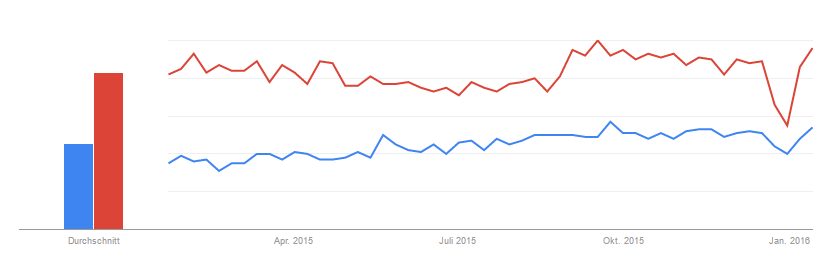
\includegraphics[width=0.7\linewidth]{figures/meteor-vs-mean.png}
	\caption{Vergleich der Suchanfragen von Meteor gegenüber Mean. Datenquelle: Google Trends \cite{googleTrends:meteorVsMean}}
	\label{f:mean-frameworks:meteorVsMean}
\end{figure}

MeteorJS wird von einigen als zukunftsträchtige Technologie in diesem Sektor gesehen.
Ob dies tatsächlich der Fall ist ist aber sehr umstritten.
Google Trends spiegelt dies in der Abbildung \ref{f:mean-frameworks:meteorVsMean} nicht wieder.